\documentclass[12pt, a4paper]{article}

\usepackage[T1]{fontenc}
\usepackage[utf8]{inputenc}
\usepackage{libertinust1math}

\usepackage{csquotes}
\usepackage[english]{babel}
\usepackage[backend=biber, style=apa, sorting=nyt]{biblatex}
\addbibresource{thesis.bib}

\usepackage{graphicx}
\usepackage{subcaption}
\graphicspath{{./assets/}}

\title{Cross-posting gamers on Reddit: An analysis of the gamer community}
\author{Joshua Megnauth\\[1cm]{\small Advised by Dr. Charles J. Gomez}\\[1cm]{\small Queens College, City University of New York}}
\date{\today}

\begin{document}
\maketitle

\section{Introduction: Reddit, gamers, and social networks}
Gaming is an omnipresent artistic medium enjoyed by a plurality of Americans. Research from the \textit{Entertainment Software Association} (E.S.A.) has found that about 65\% of American adults play video games. About 46\% of said gamers are female (\cite{esagamers}). The E.S.A.'s research counters the tired trope of gamers as young, immature boys. Despite the prevalence and diversity of gamers academia is woefully behind on ludology, the study of gaming. Gaming lacks the prestige of other artistic entertainment media such as books, music, and film. An interested party may find texts on the innovations of Allen Ginsberg's poem \textit{Howl} or Sonic Youth's \textit{Daydream Nation} while scarcely finding an academic article on the contributions of the video game \textit{Doom}.

Ludology is as exciting as fields such as A.I. despite lacking the selfsame effervescence. In other words, ludology may be studied from many different angles. Political sociologists would find much to mine from the philosophical schisms in the gaming community. Recent grassroots movements to push for more representation in video games spawned a revanchist and sexist counter movement. Besides the political, sociologists may write ethnographies of the online communities or interactions that occur within gaming. Mark Chen's \textit{Leet Noob: The Life and Death of an Expert Player Group in 'World of Warcraft'} is a study of a group of gamers who tackle dungeons in \textit{World of Warcraft}. Chen writes from the perspective of both a gamer and a social scientist to apply theories such as social and cultural capital, actor-network theory, social construction, et cetera to the video game (\cite{chenwow}). The list above is clearly not exhaustive. However, I'd like to mention, as an aside, that online communities are transient; ignoring ludology risks permanently missing out on an aspect of culture.

My thesis focusses on the intersection between network science via the social network Reddit and video games. I am particularly interested in the distribution of gamers across subreddits as well as homophily. Reddit and the related terminology will be explained below. I hypothesize that gamers are more likely to post on multiple gaming subreddits (that is, gamers are more likely to have communities that span across subreddits). Analyzing the network dispersion of gamers is useful for both the social sciences as well as marketing. Network science is concerned with the spread of information by virtue of its focus on ties. Users who post on multiple subs may transfer information across subreddits. The graph of gamers may be small world---that is, posters may be relatively well connected to rather than having to "travel" far across Reddit to encounter each other.

My guiding principle is thus to use my statistical and computing skill coupled with my domain knowledge of video games in order to contribute to ludology. Previous studies on gaming lack domain expertise while exhibiting logical fallacies---both of which seem to be caused by the hermetic world of academia. More proper ludology needs to seed the field until the study of video games resembles writing on music or films. My project requires both scraping as well as analyzing data.

An anecdote engendered my thesis. I've observed; anecdotally, like many others; that nerds of a feather tend to flock together. Gamers tend to share a sample from a common set of interests such as anime, wrestling, technology, certain tastes in music, et cetera. This observation is far from holistic---meaning, gamers do not adopt all of the same traits, and clearly not every person who watches wrestling, for example, is a gamer. However, the basic observation led to my thesis. Gamers may preferentially attach to other gamers or to other ostensibly related subjects such as anime or eSports. Either conclusion---that gamers preferentially attach or not---is useful for ludology. My research is not seeking to answer that question specifically, but my thesis may provide the groundwork toward studying that larger topic. My thesis specifically focusses on examining how gamers group together (or don't) based on related gaming subreddits.

\section{Research question}
How are gamers distributed across Reddit? Do gamers connect across subreddits on similar types of subreddits? My question, as mentioned above, aims to determine the shape of the "gamer network" on Reddit. Preliminary results have found that many gamers post across multiple gaming subreddits which may increase information dispersion. My research is limited in many ways due to time and computational constraints. Further research should seek to analyze a larger network with more similarity metrics. However, early research is encouraging in many ways as explained in the results and discussion sections.

\section{Background: social network analysis}

\subsection{A digital approach}
My goal is to contribute to both ludology as well as studies of Reddit. Gaming by virtue is a heavily technological affair. Gamers are often only lightly insulated from technology. For example, anyone who follows gaming news would likely run into computer terms. Even gamers who do not follow gaming news would run into patches, lag, bugs, or have to know how to connect their consoles to the internet, et cetera. Gaming is unlike television or cable in that video games have a strongly "digital native" feel---especially for P.C. (computer) gamers. Gamers discuss video games online on platforms such as Reddit or news sites with forums and comment systems. The culmination of these "techy" qualities does not imply that all gamers are computer scientists but that they are generally reasonably comfortable with technology. All of this is to say that a network analysis focussing on gamers and Reddit is sensible because of the focus on internet media.

\subsection{Why video games?}
Gamers and ludology, as discussed earlier, are legitimate areas of study that are largely ignored by academia as well as having an image problem regardless of gaming's prevalence. Gaming as a medium is sometimes strangely maligned as coercing individuals toward violence. In 2019, President Donald Trump as well as Kevin McCarthy and Dan Patrick, both Republican politicians, scapegoated video games as reported by an article in the New York \textit{Times}. The article explains that games are often blamed for shootings despite the lack of causal evidence. The American Psychological Association, according to the \textit{Times}, is that video games and violence are not linked. Dr. Chris Ferguson of the A.P.A. humorously mentioned that the data linking bananas to suicide are about the same as those data connecting video games and other media to violence (\cite{drapernyt0819}).

Most research published on gaming is cursory while also lacking domain knowledge on the subject. A search through databases that compile articles, such as JSTOR, on video games shows that research is decidedly lacking in imagination as they mostly focus on the antiquated violence question. One such article published in \textit{Frontiers of Psychology} exhibits a very flawed methodology in studying gamers. The researchers use an imbalanced and relatively small random sample that skews young and male. Females consisted of a scant 15\% of their sample. The writers justified the skewed sample by referencing a two decade old paper despite publishing their article in 2019 and using recent sources otherwise (\cite{badresearch}). Research from the NPD Group corroborates what the E.S.A. found and gamers already know: about half of gamers are women and more females own the 3DS, Wii U, and Nintendo Switch than males (\cite{npdgamers}). Beyond the poor sampling the research heavily relies on p-values without associated effect sizes. Furthermore, the basis for the study is intrinsically flawed. Gamers are a wide social unit. We would not sample around 3000 music buffs in order to see if "problematic music listening" is associated with "poor psychological functioning."

\subsection{What is Reddit?}
\begin{figure}[ht!]
  \centering
  \begin{subfigure}[b]{0.4\linewidth}
    
\includegraphics[width=\linewidth]{reddit_rust_comments.png}
    \caption{Comments on an /r/rust thread}
  \end{subfigure}
  \begin{subfigure}[b]{0.4\linewidth}
    
\includegraphics[width=\linewidth]{reddit_ps4.png}
    \caption{/r/ps4 threads (old scheme)}
  \end{subfigure}
  \begin{subfigure}[b]{0.4\linewidth}
    
\includegraphics[width=\linewidth]{reddit_pcgaming.png}
    \caption{/r/pcgaming threads (new scheme)}
  \end{subfigure}
  \label{fig:redditexamples}
  \caption{Examples of Reddit, a forum-like social network. The Rust programming language, PlayStation 4, and P.C. gaming subreddits are shown.}
\end{figure}
Reddit is a social network reminiscent of the forums and bulletin board systems (B.B.S.) of the past. Reddit is designed for lengthy deliberation, or at least facilitates it, which is like forums and unlike Twitter or Facebook. Subreddits is Reddit parlance for a community which is similar to a forum. Pseudonymous users may post or reply to discussion topics. Like forums, topics may be anything that fits the theme of the subreddit. For example, a subreddit on cats would have topics on cats. Individual subreddits are moderated by screened volunteers from the community; rules are enforced and users may not be able to post if their reputation---known as karma---is too low. Individual topics, known as \textit{submissions}, are also voted up or down. Needless to say, Reddit's structure engenders higher quality content in comparison to Facebook or Twitter---generally speaking at least as Reddit is also home to lengthier discussions on puerile matters. Reddit users, who are pseudonymous, are known by the demonym Redditors.

Reddit reflects gaming's preeminence via \textit{many} the many subreddits on the topic; individual consoles, series, genres, abstruse memes, as well as technological concepts such as emulation all have incredibly active subs. Reddit is the seventeenth most popular site in the world according to \textit{Alexa}, a subsidiary of Amazon that collects internet data. The social network's position varies from day to day but remains consistently high. Reddit is ahead of several prominent sites such as Netflix, Hulu, Crunchyroll, Instagram, Microsoft's site, Live (Outlook), Twitch, Bing, eBay, AliExpress, and others. Reddit is mainly behind sites such as Chinese social networks such as Weibo as well as Google and YouTube (\cite{alexatop}). The largest gaming subreddit on Reddit, \textit{/r/gaming}, is the fourth most popular total which places \textit{gaming} above the subreddits for music, sports, relationships, movies, news, gifs, cats, cute pictures, books, programming, et cetera. In fact, the only subreddit more popular than \textit{gaming} that is \textit{not} a default subscription is \textit{/r/funny}. The subreddit for \textit{League of Legends}, a single video game, is the sixtieth most popular subreddit (\cite{redditlist}).

Redditors may post on as many or as little subreddits as they wish. For example, a user may post on the subreddits for PlayStation 4, P.C. gaming, Linux, and the systems programming language, Rust. Another user may frequent the subs for K-Pop, anime, and the Nintendo Switch. The distribution of these users in terms of where they post is not obvious. In other words, a PlayStation 4 gamer does not necessarily post on the general gaming subreddit nor the subs for other Sony consoles. Redditors who post on multiple subs are part of each community. Thus, the dispersion of gamers, as discussed earlier, is a unique sociological problem. Gamers may be isolated within the specific subreddits they frequent the most or they may be distributed across a wider area.

Reddit is often considered a "news aggregator" like Slashdot, Digg, or StumbleUpon. The latter two are dead while Slashdot, a technology news site, is still alive despite predating Reddit, Digg, and StumbleUpon by over a decade.The researcher personally categorizes Reddit as a forum replacement due to the emphasis on discussions and comments rather than solely existing as curated news (\cite{tbower_2011}). However, the reader should understand that Reddit bares a lot of similarities to such services. Reddit's tag line is the "Front Page of the Internet" which implies the service is a portal to content. The content is pulled from a user's own subscriptions to subreddits. Thus, a person may have a front page with the latest political happenings, Linux news, anime discussions, et cetera.

\subsection{Very basic network definitions}
Network theory focusses on the connections between nodes. Nodes are defined based on context. Nodes in a network of friends would refer to each person. Reddit networks may define nodes as each individual account or poster. Nodes are connected to other nodes via edges. Like node, the term edge is contextual; two friends would share an edge in a friendship network. Edges may be directed or undirected. Consider a video game lending network. The edges may reflect the number of titles loaned. We can define the edge between lender and borrower as directed to account for the relationship where lender is loaning \textit{N} games out to the borrower.

Graph theorists derive many ideas of relationships as well as formulas and algorithms from this basic concept. We may sum the count of edges a node has to derive degree. The ratio of a node's degree to its potential degree is known as degree centrality (importance). Degree centrality is intuitive because we're calculating a ratio of connections. Thus, more connected nodes would have a higher degree centrality. Nodes traverse paths to reach other nodes. A path exists between two nodes (A, B) if A may cross a sequence of edges to reach B. Additionally, paths only traverse a node or edge once. Betweenness is a metric that measures how often a node is on the shortest path between two nodes. Logically, a node that other nodes often traverse to reach some destination is important in some way (consider airlines or chiefs of staff). A relationship of three nodes creates a triangle or triad. The ratio of triads to potential triads provides a metric for average clustering.

Network theory is obviously more complex than the simple one line, non-mathematical definitions above. However, the basic definitions should suffice for now. Interestingly, some definitions and formulas in the network community seem disputed. Some problems, such as community detection, lack elegant solutions.

\subsection{Big data---Volume, Variety, and Velocity}
Graph theory does not imply big data, but network science scales well to a high number of observations.Computational social science naturally trends towards big data, such as large graphs or natural language processing. Amir Gandomi and Haider Murtaza argue that the term "big data" is often misunderstood which may impact comprehending a big data project. Big data is traditionally defined by the three Vs: volume, variety, and velocity. Volume is the most straightforward of the three concepts. The "big" in big data suggests a generous amount of information. Volume is simply that---\textit{a lot} of data (\cite{gandomiamir2015}).

Variety and velocity are the more interesting of the three Vs. Big data is often raw and heterogeneous. Unlike the nicely structured flat files data are often distributed as, the majority of existing data are unstructured and multiformat (\cite{gandomiamir2015}). For example, Twitter data would likely arrive in a set of different languages with varying levels of grammar, zeitgeist and context specific references, embedded multimedia, retweets, et cetera. With that said, Twitter data may still be pulled from a clean API which means that Tweets are hardly the most unstructured data a scientist would find. Variety, thus, also refers to the format of data; different image or video formats must be handled, and unstructured data must be appropriately stored as well.

Big data is not only intractably diverse but they are also produced at a high velocity (\cite{gandomiamir2015}). For example, consider all of the data gathered by voice processing systems such as Watson, Siri, Alexa, or Google Assistant. Simply browsing the internet, even with JavaScript and DNS blocking, produces an enormous amount of data. Cellphones collect data more or less constantly, especially with more programs/apps in use. \footnote{Data are collected in a manner so megalomaniacal that the European Union instituted the \textit{General Data Protection Regulation} to protect the privacy of E.U. citizens.}

The three Vs galvanized the use of certain techniques of gathering and analyzing data. Natural Language Processing, graph theory, unstructured databases, clustering, et cetera are not new, but big data have made such techniques both more viable as well as more necessary. NLP, neural networks, as well as computer vision are hotshot fields of data science more generally as well as the computational social sciences due to the prevalence of so much data. After all, what else would we do with said data (\cite{gandomiamir2015})?

Social network analysis is at least a century old, but big data presents new applications according to Gandomi and Murtaza. Modern S.N.A. is "data-centric" due to the "growing adoption" of social media as well as the many platforms in use. Computational social scientists may analyze either the content or structure of social media data. Network analysis is structural as the \textit{ties} between posters are analyzed. For example, social scientists may use community detection to uncover hidden structures in networks, such as coposters or citation flows for research. Social network analysis may also discover the nodes that are most influential in a network or predict potential links between nodes. Big data's prevalence as well as the massive networks that are common today are driving research into social networks (\cite{gandomiamir2015}).

\subsection{Weak ties in social networks}
Mark Granovetter's "Strength of Weak Ties" is a sociological classic that argues that micro level "interpersonal ties" affect macro level phenomena. Granovetter defines a small network consisting of two nodes, \textit{A} and \textit{B}, and their friends and acquaintances. Strong ties tend to create other strong ties. For example, \textit{A} and \textit{B}'s respective close ties would likely meet \textit{A} or \textit{B} as well. Nodes in a network transfer information so that our two nodes and their ties gain information from each other. As a small note, Granovetter uses "information" laxly to refer to anything that may be transmitted diffusely, such as knowledge or even disease (\cite{granovetter1973}).

Information transfer is not limited to strong ties. Granovetter explains that weak ties act like "bridges" that create shortest paths for information to flow. Strong ties act as amplifiers that repeat and retain information. For example, consider \textit{A} and \textit{B}'s close ties. Rumors, jobs, feats of excellence or failure would all be retained within the strong ties of the network since information is constantly echoed throughout the clique. Weak ties, on the other hand, are "highways" that transmit information rapidly and across distances too. A network of only strong ties is isolated and disjointed. Granovetter uses several examples, including disease; we can consider COVID-19. The coronavirus spread through a series of coincidental ties that eventually made way into areas of stronger ties. In other words, COVID-19 couldn't spread through strong ties alone as that would be too slow. Weak ties diffuse information in general such as jobs, rumors, new ideas, et cetera. Discoveries or new inventions spread easier through networks containing a lot of weak ties due to the heterogeneity of such a network (\cite{granovetter1973}).

Granovetter theorized that people with similar tastes have a pull to form ties. To repeat Granovetter, let's say that Node \textit{A} and \textit{B} are friends and node \textit{C} is friends with \textit{A} but not \textit{B}. Nodes \textit{B} or \textit{C} would be compelled to form ties with each other (\cite{granovetter1973}).

Reddit is strongly attuned to the idea of weak ties. Redditors likely do not post in subreddits consisting of only close ties. Strangers, or at least mild acquaintances, hold topics and discussions on Reddit. Posters may recognize certain Redditors over time, but the connection is still tangential rather than strong. The "velocity" and "volume" of information produced on Reddit facilitates creating weak links as well as information transfer. Some critics contend that the power of weak ties is often exaggerated. Weak ties require some strength behind them to have effect rather than having an effect by default (\cite{kadushin2011}). Reddit's weak ties have some force behind them due to the focus on discussions. For example, many topics hold in depth conversations on music, films, video games, politics, relationships, computers, et cetera. New games or albums may rapidly traverse the relevant areas of Reddit if popular enough. Such mechanisms operate on Twitter too, of course, but Reddit is specifically geared toward longer communication which in turn holds more power than a couple of characters. Reddit, unlike Twitter, is not full of fake users and bots that hinder rather than improve connectivity.

\section{Structural holes}
Ronald Burt extends the weak ties metaphor by arguing that nodes or people near structural holes are more likely to have good ideas. Structural holes are nodes or empty spaces where two different networks meet. Structural holes represent the potential for action. Actors near structural holes may potentially transfer information across networks. Burt argues that the right network conditions must be met with ingenuity. In other words, the bridge or edge must be recognized and then formed. Burt claims his research lacks "novelty" but instead expands ideas that other social scientists have previously laid out in some shape or form. Both Adam Smith as well as John Stuart Mills believed that associating with the "dissimilar" broadens a person's mind. Other social scientists, such as the philosopher Friedrich Hayek, explained how economies integrate over segments (holes) where actors have specialized skills. Burt explains that the general theme of the works of the many disparate writers he covers is that "information, broadly conceived, are more homogeneous within than between groups." Fundamentally, Burt's basic idea is radical for synthesizing ideas previously stated by philosophes like Mills or Hayek into network theory (\cite{burt2004}).

Consider two networks of corporations where one network consists of food production businesses and the second encompasses data scientists who work in computer vision. A business that resides on the periphery of the two networks or at least has connections to both networks is near a structural hole. The business near the hole may transfer expertise across the networks like Granovetter's bridge edges. Good or novel ideas may arise from the business uncovering areas where the networks may converge---such as using computer vision to improve farming.

The same concept applies to Reddit albeit more abstractly. Structural holes exist near the boundaries of related subreddits. Subreddits do not have \textit{actual} boundaries separating them of course. However, related subs contain information that may be dispersed through weak ties. For example, a user may ask a question about a video game on a general sub that is answered on a more specific sub or vice versa. Users who read both subs are able to direct the questioner appropriately. Readers of multiple subreddits integrate their knowledge into those same subs as well as gain insights from each sub. If the poster writing the inquiry reads multiple subs themselves they will be more likely to encounter an answer. Thus each poster in each sub constitutes a weak tie to each other poster. The potential information available to a poster in a single sub is thus that of the respondents which in turn spans all of the subs visited by said respondents. In other words, weak ties in subs are potentially projected across all readers. The access to information involves relatively little hops.

One flaw of the concept above is that we are considering an ideal manifestation of weak ties. Weak ties are important in terms of their bridging capability as per Granovetter. A weak tie may not act as a bridge and thus not transfer information. In our example above, posters who may have answers to questions or tips for the game at hand from other subreddits or experience do not have to share their knowledge. A more nuanced view of weak ties takes into account that posters aren't abstract nodes or machines but must have the willingness to act or the ability to actually arrive at an insight as covered above in the Granovetter section.

\subsection{Co-posting networks via Reddit}
While studies of Reddit are rather rare, researchers tend to be inclined towards studying \textit{co-posting networks}. Co-posting is essentially a type of propinquity---or residing in the same "space" where space is defined by the topic or researcher. Space in the sense of co-posting refers to residing in the same topic or subreddit. For example, every poster on a specific topic ("I'm struggling to beat \textit{x} boss. Please help!") would be co-posters. Co-posters may also be defined as all posters on a subreddit such as \textbf{/r/KingdomHearts}.

Troy Steinbauer's 2010 paper on Reddit co-posting networks is one of the earliest studies of the social network. Steinbauer gathered submissions and comments from the top 1\% of subreddits at the time as well as general data on Reddit. The average subscriber count for subs total at the time of his analysis was about 1077 with a +1 standard deviation of 23514---extremely wide as well as skewed. His research analyzed related subreddits, comment trees, and friend graphs. 2010 is ancient in terms of computational social science, but Steinbauer's methods are still useful for my study (\cite{tbower_2011}).

\begin{figure}[ht!]
  \centering
  \begin{subfigure}[b]{0.4\linewidth}
    
\includegraphics[width=\linewidth]{related_pcgaming.png}
    \caption{Related subs /r/pcgaming}
  \end{subfigure}
  \begin{subfigure}[b]{0.4\linewidth}
    
\includegraphics[width=\linewidth]{related_ps4.png}
    \caption{Related subs /r/PS4}
  \end{subfigure}
  \caption{Examples of "related subreddits" via two gaming subs.}
\end{figure}

Subreddits may link to other "related" subs as decided by the owners. A related sub is whatever the owners decide. For example, a subreddit on a game series may link the individual subs for each game as well as related series. Steinbauer created a graph where each node is a sub and each edge is a "related" connection between two subs. Subreddits tend to have less than fifteen related links besides a few special subs. The related subs graph is also not very well connected. The largest connected component (LCC) of the graph only contains about 25\% of the nodes while the average clustering coefficient is low at 0.039 (\cite{tbower_2011}).

Steinbauer's comment tree graph is far more connected than than his related subs network. The basis of the network is a set of thresholds for comments. Steinbauer defines a loose graph as having an undirected edge between two posters, A and B, if A or B responded to the other. A tight graph requires both posters having responded to each other. Finally, a strict graph is like a tight graph except with a threshold of four comment pairs between respondents. The final graph is remarkably connected in terms of LCC as the largest component of the loose and tight graphs contain over 98\% of the nodes while the strict graph contains about half of the nodes in the LCC (\cite{tbower_2011}).

Graham Earley, Nikita Fomichev, Willa Langworthy, and Ruyi Shen studied the Bernie Sanders and Donald Trump subreddits in 2017. \textit{A Statistical Analysis of Network Data From Reddit} is a very mature approach to network science as the researchers use natural language processing (NLP) for some of their node attributes. Earley et alia define nodes as posts to submissions. Particularly, they calculate average sentiment scores per post. The median length of posts is longer on the Sanders sub in comparison to the Trump sub. Posts on the Sanders sub tend to be longer for all three sentiment categories studied as well---positive, neutral, and negative. Positive posts on the Sanders sub sport an average length of 540.2 compared to 35.36 on the Trump sub. Neutral posts tended to be short on both subreddits (\cite{causeweb2017}).

Next, Earley et alia calculate network statistics for the two graphs. The Sanders subreddit is much more clustered than the Trump sub at .897 versus .497 for transitivity respectfully. Modularity, or the ability to subset nodes into non-overlapping sets, is also higher for Sanders' sub at .707 in comparison to .505 for Trump. Both of these imply greater connectivity for posters on the Sanders sub as they're responding to each other more across submissions. Average path length is about the same for both graphs despite the difference in clustering (\cite{causeweb2017}).\footnote{Reddit recently banned \textbf{/r/the\_donald} due to users spearheading attacks on other communities. The community's notoriety spans beyond coordinated trolling. The sub bred conspiracies and racist memes. The posters eventually fled to an echo chamber and "alternative" Reddit that respects their first amendment rights. Note that Reddit isn't a governmental organization that can violate the freedom of speech (\cite{thedonaldban2020}). I assume that the relatively disconnected nature of the sub shown in the paper may be due to the sub lacking the cohesiveness of an actual community. The Donald is more of an ideology, like \textit{juche sasang}, which in turn means the sub was closer to the puerile subs noted earlier. Users may have visited and posted memes and rants rather than engaged in substantive conversation.}

So far, we looked at research that considers nodes and edges as Redditors and posts without considering the literal flow of information. Giannis Haralabopoulos, Ioannis Anagnostopoulos, and Sherali Zeadally studied the propagation of information for Reddit, Twitter, and Facebook as well as the media services YouTube and ImgUr. They defined a metric called the Unit of Interest that measured propagation for each service above. The metric varied per service as each defines "success" differently. For example, Facebook's metric was defined as likes per post. The gathered data were filtered to preclude posts that failed to double the UoI four times. Gaming ended up as one of the most prevalent topics, especially on Reddit, after the data were filtered (\cite{haralabopoulos2015}).

\subsection{Assortativity and co-posting networks}
Assortativity is the tendency for nodes to be attracted to other nodes with similar characteristics. Both "nodes" and "characteristics" are general here---assortativity (also known as homophily) is not limited to social science. Networks with high assortativity tend to be more robust to removing nodes and edges as theorized in a seminal paper by M.E.J. Newman. Social networks tend to have higher assortativity than other types of networks. Humans naturally flock together for certain qualities such as, perhaps, politics. Computational social scientists have studied graphs of online social networks, such as Twitter, to determine if robustness holds for assortativity. The paper \textit{Co-posting Author Assortativity in Reddit} is one of the first to see if Newman's theory holds for Reddit (\cite{cauteruccio2020}).

Research by Cauteruccio, Corradini, Terracina, Ursino, and Virgili tested Newman's hypothesis for Reddit. The researchers gathered 150,795,895 observations that they used to create a co-posting network. Density is low at 0.006 which is sensible considering the wide range of data scraped. Cauteruccio et alia first calculated assortativity based on degree centrality. Posters were binned into intervals 312,500 nodes wide. The researchers calculated assortativity for the extreme intervals as well as the intermediate intervals. After comparing their results with a null model created with permutation the researchers found that posters in an interval are more likely to have more connections within their interval than outside (\cite{cauteruccio2020}).

\subsection{Community mapping and small world networks}
Computational social scientists may map out ephemeral communities using networks. Communities and roles may be \textit{emic} or \textit{etic}. \textit{Emic} refers to nominal position assigned by a group such as president or manager. \textit{Etic} refers to the actual structure as discovered by some process such as network science, anthropology, political science, et cetera (\cite{kadushin2011}). For example, an analysis of the United States government would show the relative power of the nonpartisan independent agencies that execute the law. Analyzing Reddit may reveal communities that span borders (subreddits).

The digital humanities are known for having a fuzzy definition and community due to the diverse fields of study. Martin Grandjean applied social network analysis to Twitter in order to determine the shape of the community. Grandjean gathered the users from Tweets mentioning specific hashtags, keywords in biographies, Twitter's search functionality, and volunteers who had heard of his research (\cite{grandjean2016}).

The final graph is a low density network that nevertheless exhibits small world qualities. Most users are individually weakly connected. In other words, users may have access to the entire network while not being deeply rooted in it. Language created clear clusters in the network despite inter-language connections. Languages present in Grandjean's data include English, French, German, Dutch, and Spanish. Grandjean found that users with high betweenness centrality reside at the intersection between these communities (\cite{grandjean2016}).

Self-similarity and small world are often considered two antagonistic properties. Small world graphs may not be fractal---the mathematical property of repeating as length increases. However, complex networks, such as social networks, may be self-similar depending on the subset. Gallos et alia studied a subset of the IMDB movie network that consisted only of adult film actors. The subset allowed them to use a relatively small and focussed data set that was also small world. The researchers set a threshold of co-starring connections in order to get rid of connections that obscure fractality. Some connections are relatively less important than others. Therefore, precluding those weak connections in order to reveal possible fractality is an acceptable trade. The researchers implemented a box covering algorithm that showed network fractality for the reduced graph when only stronger ties were considered (\cite{galloscuny2013}).

\subsection{Information spread in online social networks}
Information spread is something of a hot topic in terms of studying online social networks. Virality, the rise of social movements, the spread of propaganda or conspiracy theories such as QAnon, memes, information dispersion, et cetera are all phenomena that may be studied in terms of social networks. Sen Pei et alia studied determining superspreaders in networks. Superspreaders amplify messages which in turn mean they're of high importance for everything from marketing to social movements (\cite{peispread2014}).

The researchers found that algorithms like Google's PageRank perform poorer than expected. Pei et alia argue that prior papers are flawed due to the way they simulate network data to test algorithms like PageRank. These papers simulate data based on epidemiology via random walk models. PageRank, which is similar to eigenvector centrality, tends to perform well with the simulated data. However, different algorithms outperform PageRank depending on the problem. K-core performs better than PageRank for real world epidemiology data but poorly on rumor data, for example. Furthermore, simulated models fail to handle properties such as assortative mixing which occurs naturally in real world networks (\cite{peispread2014}).

K-core outperformed other algorithms based on the findings by Pei et alia. Metrics such as K-core or eigenvector centrality are global metrics that require complete networks to be properly calculated. Studying online social networks such as Reddit, Twitter, or Facebook is thus extremely difficult or perhaps impossible unless a clear subset is demarcated. Thus, they collected the entirety of the LiveJournal network in order to both circumvent the errors caused by simulated data as well as the difficulty of studying influence in other online social networks (\cite{peispread2014}).

Gathering the entire LiveJournal (LJ) network allowed the researchers to track information diffusion globally. In other words, the researchers were able to follow every link made by a user to an LJ blog other than their own. Starting with a user, \textit{i}, the researchers followed the chain of users who linked to posts by \textit{i} as well as users who linked to the links et cetera. The method accounts for every user rather than conferring importance on whichever users the algorithm picked as a starting point. The result is the influence of every user whose content was shared. K-core outperforms PageRank for the LJ data. PageRank incorporates a random walk. Random walks may work for ranking website links but for social networks performance is suboptimal (\cite{peispread2014}).

\section{Methodology}

\begin{figure}[ht!]
  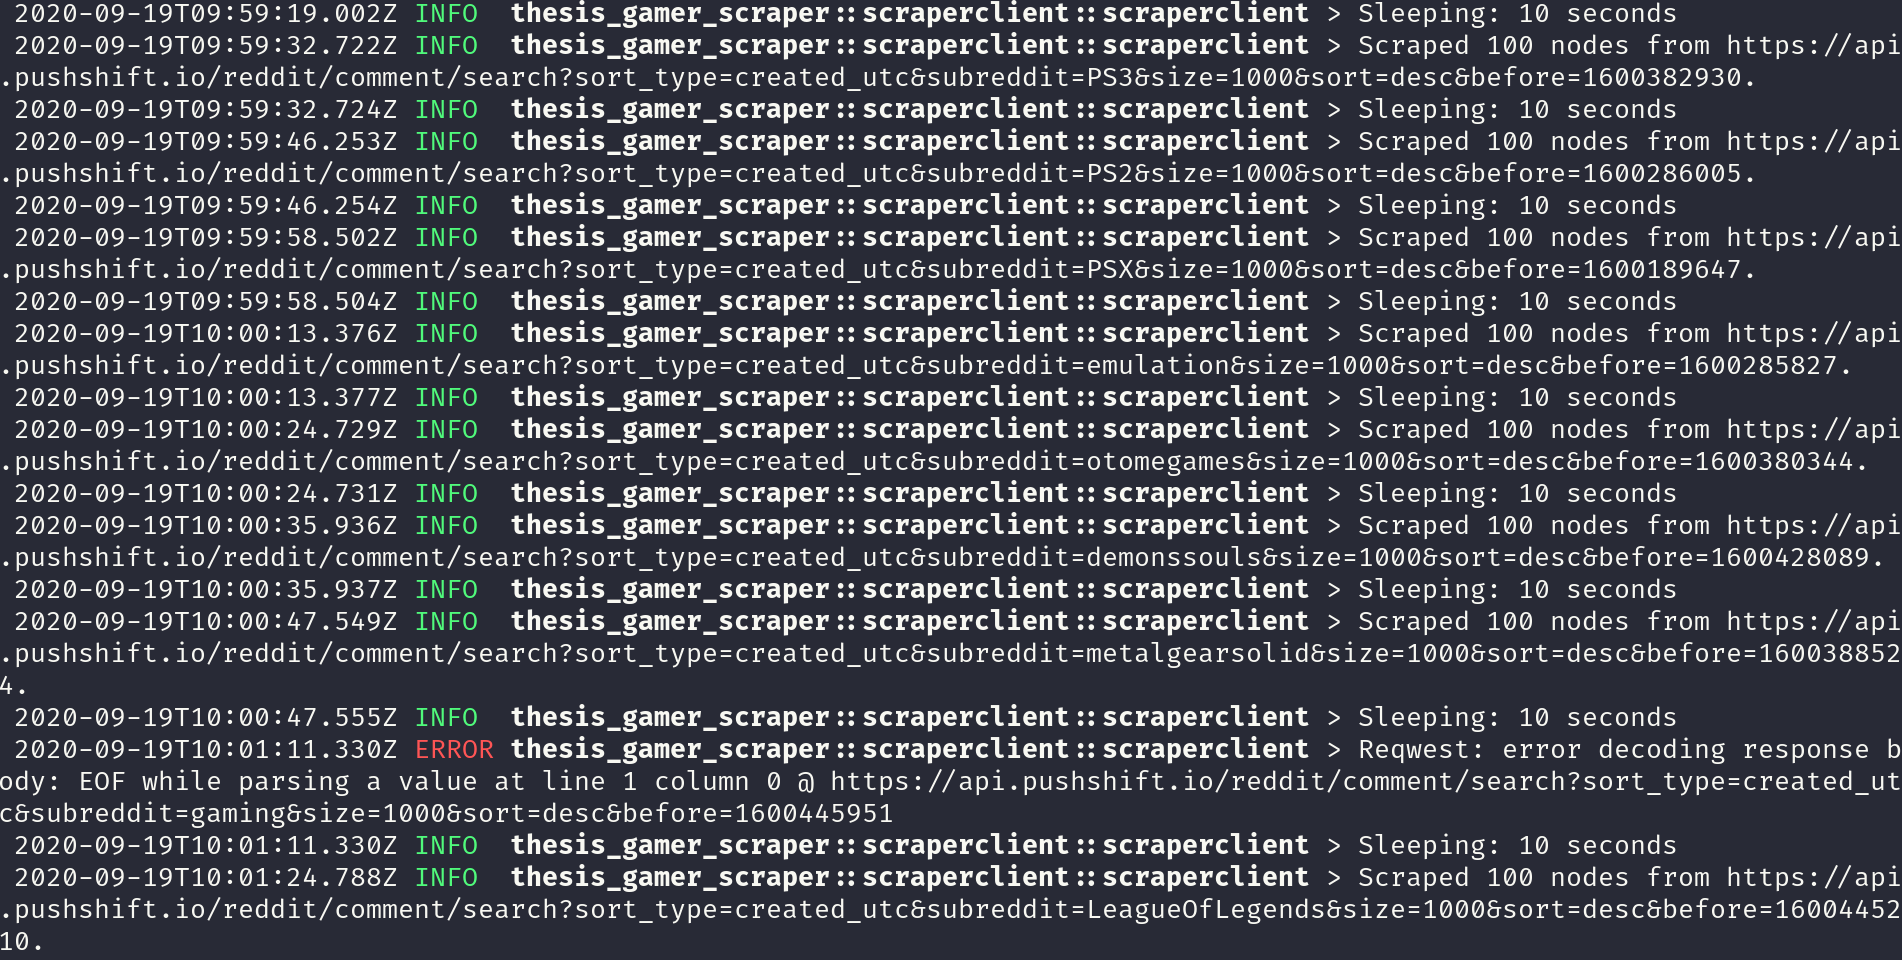
\includegraphics[width=\linewidth]{scraper_at_work.png}
  \caption{Scraper hard at work.}
  \label{fig:workingscraper}
\end{figure}

My research project requires relatively recent data as well as observations relevant to video games. Researchers in the computational social sciences seem to trend toward gathering their own data. The internet is a dynamic space of constant data production. Structured data may be limited or flawed for many topics, including ludology. Scraping data allows computational social scientists to gather raw, unpasteurized data rather than relying on old, static sources. A survey, for example, is saliently flawed for gamers because conducting one properly would likely require a large sample across a wide span of ages as well as capture gamers who play on different platforms. Scraping data seems both more reliable as well as more direct in a case like that as well as for my project.

While large Reddit data sets exist via the \textit{Stanford Network Analysis Project} as well as \textit{Kaggle}, scraping data from Reddit is not too difficult due to the open Reddit API (\cite{redditapi}). Bindings for Python exist via \textit{PRAW} as well. However, the Reddit API imposes several restrictions and requires an account to use properly as well. The restrictions are reasonable due to Reddit's high traffic: rapacious scrapers may hammer the site and associated Content Delivery Networks. Caching services, such as the open source Pushshift, aims to alleviate the stress caused by scrapers as well as provide a more convenient API (\cite{pushshiftapi}). I opted for Pushshift to gather my data due to its flexibility.

My scraper gathers \textit{N} Node-Edge pairs from a provided list of subreddits. I wrote the scraper in the systems programming language, Rust, and the source code is available on GitHub\footnote{https://github.com/joshuamegnauth54/thesis\_gamer\_scraper}. My program's high level logic is as follows:

\begin{enumerate}
  \item Collect 100 nodes with associated metadata from a subreddit. Each observation contains the Redditor name, epoch timestamps, topic, and subreddit name.
  \item Paginate by setting the \textit{before} API parameter to the earliest timestamp from the recent scrape of 100 nodes.
  \item Add each gathered node to a hash set which precludes duplicate observations.
  \item Repeat steps one through three for the set of subreddits in a round robin manner.
  \item Repeat steps one through four until \textit{N} is reached.
  \item Remove deleted users and automoderator replies.
  \item Hash all of the Redditor and topic names with SHA256 at an attempt at privacy\footnote{Very little of the data sets found online actually hashed the user names as the information is all public. However, hashing at least adds a minimum layer of privacy.}.
  \item Deserialize everything to a CSV.
\end{enumerate}

My data set\footnote{Available here: https://github.com/joshuamegnauth54/GamerDistributionThesis2020/data} contains about 127,000 observations gathered via the logic above. The first and most salient limitation here is that I only gathered 127K observations for a select set of subreddits. I originally intended to perform a breadth first search by scraping outwards from the nodes. So in that case each node in the set of unique nodes would be individually queried for the list of subreddits they posted to at least \textit{N} times to add noise to the data. Ironically, Pushshift lacks an easy access point (as far as I know) for gathering those data. My program contains the requisite logic to scrape that data from Reddit without using their API\footnote{See: https://github.com/joshuamegnauth54/thesis\_gamer\_scraper/blob/master/src/scraperclient/scraperclient.rs The \textit{scrape\_individ\_users} function implements the logic.}, but Reddit bans users who are caught scraping data outside of their public API.

My analysis uses the open source Python\footnote{https://python.org} library NetworkX (\cite{networkx}). Python is an interpreted, high level general purpose programming language. In short, Python is powerful and fast to write. NetworkX is a native Python library that implements an impressive collection of graph algorithms including random graph generators. Alternatives include igraph, a C library with Python and R bindings; and petgraph, a Rust crate. NetworkX sports an easy and pragmatic API but is also far slower than libraries written in speedy systems languages. Besides NetworkX, GraphViz and Pandas, both open source, were used for auxiliary tasks such as visualizations as well as wrangling my raw data. The source code for the analysis is located in the same repository as the thesis itself\footnote{Here: https://github.com/joshuamegnauth54/GamerDistributionThesis2020/tree/master/src/pyport}.

\subsection{Limitations}

Big data tend to be intractable due to the three Vs as discussed earlier. Many tests and algorithms are difficult to comfortably run on single computers even if said machines sport excellent hardware. Average node connectivity, average shortest path, betweenness centrality, small world sigma, and other useful metrics are extremely slow to calculate for two reasons. The first issue is that many of the algorithms are highly complex and balloon in running time contingent on how many vertices and edges are present. In other words, many of the algorithms used have a multiplicative or exponential time complexity. NetworkX, despite its repertoire of algorithms and general excellence, is known for being relatively slow compared to other graph implementations. NetworkX is a pure Python library (\cite{networkx}). Python is considerably slower than fast, compiled languages; this is the tradeoff interpreted and scripting languages face. Libraries such as Pandas for data frames/tabular data make use of NumPy, a wrapper around low level linear algebra libraries. Pandas mitigates the slower speed of Python via NumPy. However NumPy is an optional dependency for NetworkX which is only used for some algorithms if requested which in turn means that NetworkX can be very slow. I still wrote my code using NetworkX because the API is Pythonic and treats Python as a first class citizen. Thus, I focussed on the problem domain with the clear negative that my run times were unwieldly.

Notably, other authors, such as Cauteruccio et alia, ran into computational issues as well. Those researchers solved their problem by using server caliber hardware to run their code and calculations. Future research into the distribution of gamers on Reddit would require both vastly more data as well as more powerful hardware to handle those data.

\subsection{Network processing}
\begin{table}
  \centering
    \begin{tabular} {c c c}
      \hline \\
      Subreddit & SysGamGen & Systems \\
      \hline \\
      DarkSouls2 & Game & Multiple \\
      KingdomHearts & Game & Sony \\
      darksouls & Game & Multiple \\
      fireemblem & Game & Nintendo \\
      MonsterHunter & Game & Multiple \\
      Doom & Game & Multiple \\
      bloodborne & Game & Sony \\
      DevilMayCry & Game & Multiple \\
      darksouls3 & Game & Multiple \\
      pokemon & Game & Nintendo \\
      halo & Game & Microsoft \\
      yakuzagames & Game & Sony \\
      Fallout & Game & Multiple \\
      DestinyTheGame & Game & Multiple \\
      metalgearsolid & Game & Multiple \\
      skyrim & Game & Multiple \\
      monsterhunterworld & Game & Multiple \\
      demonssouls & Game & Sony \\
      wow & Game & P.C. \\
      MineCraft & Game & Minecraft \\
      Overwatch & Game & P.C. \\
      GlobalOffensive & Game & P.C. \\
      leagueoflegends & Game & P.C. \\
      DotA2 & Game & P.C. \\
      zelda & Game & Nintendo \\
      AnimalCrossing & Game & Nintendo \\
      witcher & Game & Multiple \\
      PUBATTLEGROUNDS & Game & P.C. \\
      SEGA & Game & Multiple \\
      smashbros & Game & Nintendo \\
      RocketLeague & Game & Multiple \\
      FallGuysGame & Game & Multiple \\
      StarDewValley & Game & Multiple \\
      psx & System & Sony \\
      PS3 & System & Sony \\
      ps2 & System & Sony \\
      pcmasterrace & System & P.C. \\
      nintendo & System & Nintendo \\
      xboxone & System & Microsoft \\
      pcgaming & System & P.C. \\
      PS4 & System & Sony \\
      Steam & System & P.C. \\
      buildapc & System & P.C. \\
      NintendoSwitch & System & Nintendo \\
      PS5 & System & Sony \\
      XboxSeriesX & System & Microsoft \\
      3DS & System & Nintendo \\
      xbox & System & Microsoft \\
      xbox360 & System & Microsoft \\
      JRPG & General & Multiple \\
      gamedesign & General & Non-system \\
      linux\_gaming & General & Non-system \\
      otomegames & General & Multiple \\
      boardgames & General & Non-system \\
      emulation & General & P.C. \\
      Games & General & Non-system \\
      gaming & General & Non-system \\
      GamePhysics & General & Non-system \\
      rpg & General & Non-system \\
      truegaming & General & Non-system \\
      ShouldIBuythisgame & General & Non-system \\
      FreeGamesOnSteam & General & P.C. \\
      IndieGaming & General & Non-system \\
      \hline
    \end{tabular}
    \caption{Listing of two main assortativity measures. SysGamGen is shorthand for Systems, Games, and General.}
    \label{tab:AssortSplit}
\end{table}
Like all data my network required processing and cleaning. Likewise, data processing should be disclosed for reproducibility. I pruned my network by removing nodes that appear less than three times. The value three is somewhat arbitrary as I intended to maximize the number of observations kept while removing a good chunk of the noise. A threshold of three did not shrink the network unreasonably; the majority of the data remained and manageability increased.

Next, subreddits were divided into two assortativity or similarity measures shown in table \ref{tab:AssortSplit}. The subs themselves were compiled in large part based on Mike Sizz's Reddit List by manually selecting the top gaming subs (\cite{redditlist}). Prior knowledge guided creating the assortativity classes. Nodes are assigned based on the sub that they posted in most frequently. Separating the subreddits by \textit{Systems, Games, and General} or each console feels naturalistic. \textit{Systems, Games, and General} classifies subreddits by whether they refer to a system (such as all subs for all consoles or P.C.s), relate to a game, or are about general purpose gaming. The \textit{Systems} distinction is similarly natural. Some subreddits are simply more associated with a specific console or company than others. For example, Mario, Zelda, Animal Crossing, Metroid, et alia are Nintendo only series. I took some liberties with series that are generally associated with a platform but have only recently become multiplatform. The Yakuza series is a quintessential PlayStation series. However, Sega recently (2019 and beyond) ported the series to P.C. Likewise, Halo is an Xbox series that 343 Industries recently ported to P.C. (2018\footnote{For the \textit{Master Chief Collection}. The first two Halo games had older P.C. ports, but Halo was still commonly thought of as an Xbox series.}) I classified these two series under their respective original platforms due to data limitations. Data limitations affect classifications in other ways as well. Gathering even more subreddits would open more potential classes. For example, perhaps genres and games would be a viable metric if I were able to scrape more data.

\subsection{Graph projection}

My network data contain two different paths for projection. Network data may be bipartite which means that nodes may be separated into disjoint sets (\cite{banerjee2017}). In other words, a network is bipartite if you can split it into, for example, node sets \textit{A} and \textit{B} where nodes in \textit{A} only connect to \textit{B} and not to \textit{A} and vice versa. For my network data, Redditors post to topics which reside in subreddits. Topics do not have edges with other edges in this scheme and likewise for Redditors. However, I am interested in the relationships between posters which means that the bipartite network must be projected in order to generate edges between posters.

Bipartite graphs may be projected to create logical edges between nodes in one of the node sets. I project topics unto authors so that every Redditor who posted on a topic now shares an edge with other posters in that same topic. Logically, everyone who posted on a topic naturally shares a connection. My data also contain subreddit information to use for projection. However, subreddits seem too coarse as a top node which in turn leads to far too many spurious edges. While all posters on a subreddit naturally share a connection, I opted for a more granular and robust connection via topics.

\subsection{Python code and metrics}

My code is fully available on GitHub as well as my data for replicability. The file \textbf{main.py} contains functions showing how I called the other functions I wrote. I loaded and processed my data using the convenience functions in \textbf{gamenetloader.py}. The files \textbf{projections.py} and \textbf{gamenetattrs.py} contain small, pithy functions that wrap NetworkX functions for graph projections and adding attributes. In terms of plotting, \textbf{gamersdraw.py} and \textbf{pvalueplots.py} contain the code used for the plots below. The plotting functions are somewhat generalized and have been used for unrelated data via another project. Those routines customize the plots by pulling out specified attributes or applying a statistic such as degree centrality. For example, network scientists often color or change the size of nodes to indicate the value of a metric. Larger nodes represent higher values of the statistic. I also wrote functions to aide in drawing k-core graphs as well as plots for random graph replicates. The code is fairly commented and hopefully easy to follow.

I calculated radius, diameter, average clustering, density, degree assortativity, and assortativity for SysGamGen and Systems using NetworkX. Radius and diameter revolve around the idea of eccentricity or the distance between a vertex, v, and the set of all vertices in a graph. The radius (or center) is the set of nodes with minimum eccentricity while diameter consists of the nodes with maximum eccentricity. Radius and diameter measure closeness. The radius of a network would show the nodes which are closest to all other nodes. For my network, radius and diameter are interesting in terms of potential information dispersion. Central posters may reach other users more easily whereas nodes in the diameter may be more difficult to reach. Betweenness and closeness centrality are both ideal metrics that are unfortunately impossible to calculate due to the limitations mentioned above.

Average clustering is the ratio of observed triangles to total possible triangles. A triangle, or triad, is a relationship where three nodes share edges so that they are all connected and form a triangle. Triangles are important in terms of social ties as Granovetter argued as people tend to form triads based on similar tastes and feelings. Density is a related statistic that measures the ratio of observed edges to the count of possible edges. A dense network is well connected due to the amount of existing edges. Large scale online social networks are likely to be more sparsely connected due to the diversity of communities as well and their spread. High densities are not always desirable.

Assortativity (or homophily) is the tendency for nodes to connect to nodes alike in some way as briefly mentioned above. For example, gamers with PlayStation may be more likely to post on subreddits related to PlayStation or PlayStation games. I calculated degree assortativity and attribute assortativity using NetworkX. Degree assortativity is homophily based on similar degree or amount of connections. Attribute assortativity is the concept mentioned above where nodes are tested on their connectivity based on a quality held in common.

\subsection{Random graph replicates}

I calculated p-values via random graph replicates using the process defined in \textbf{randomnet.py}. Process:

\begin{enumerate}
  \item Generate a random bipartite graph with the same number of top nodes, bottom nodes, and edges as my \textbf{unprojected} graph
  \item Project graph to mimic the observed network
  \item Calculate a statistic using that projected graph
  \item Repeat the steps above 10000 times using multiprocessing to speed up calculations
  \item Repeat for each of the desired statistics
\end{enumerate}

The steps above produced 10000 replicates of average clustering, density, degree assortativity, and attribute assortativity on SysGamGen.

\section{Results}
\begin{table}
\centering
  \begin{tabular} {c c c}
    \hline \\
    Metric & Full network & LCC \\
    \hline \\
    Nodes & 11474 & 11203 \\
    Edges & 170120 & 170080 \\
    Radius & $\infty$ & 1 (122 default) \\
    Diameter & $\infty$ & 2 \\
    Clustering & 0.03297 & 0.03372 \\
    Density & 0.00258 & 0.00271 \\
    Degree assortativity & 0.17329 & 0.173 \\
    Assort (SysGamGen) & 0.78194 & 0.7819 \\
    Assort (Systems) & 0.74587 & 0.74581 \\
    \hline
  \end{tabular}
  \caption{Network and LCC statistics calculated via NetworkX.}
  \label{tab:NetworkStats}
\end{table}

Preliminary results are rather interesting despite the limitations discussed above. The calculated statistics are available in table \ref{tab:NetworkStats}. The full weighted projection of the graph contains 11474 nodes and 170120 edges. The LCC, surprisingly, is barely reduced at 11203 nodes and 170080 edges (that is, only 40 edges smaller). In other words, data collection pulled hundreds of individuals who appeared repeatedly in the data (which is evident from the processing discussed earlier) who also responded to other users across topics enough to ensure that the network has a large LCC. LCC is not density or transitivity, but enumerating connected components helps observe connectedness. The connected components smaller than the LCC are all of a small length, such as one or two nodes with degrees of one.

\begin{figure}[ht!]
  \centering
  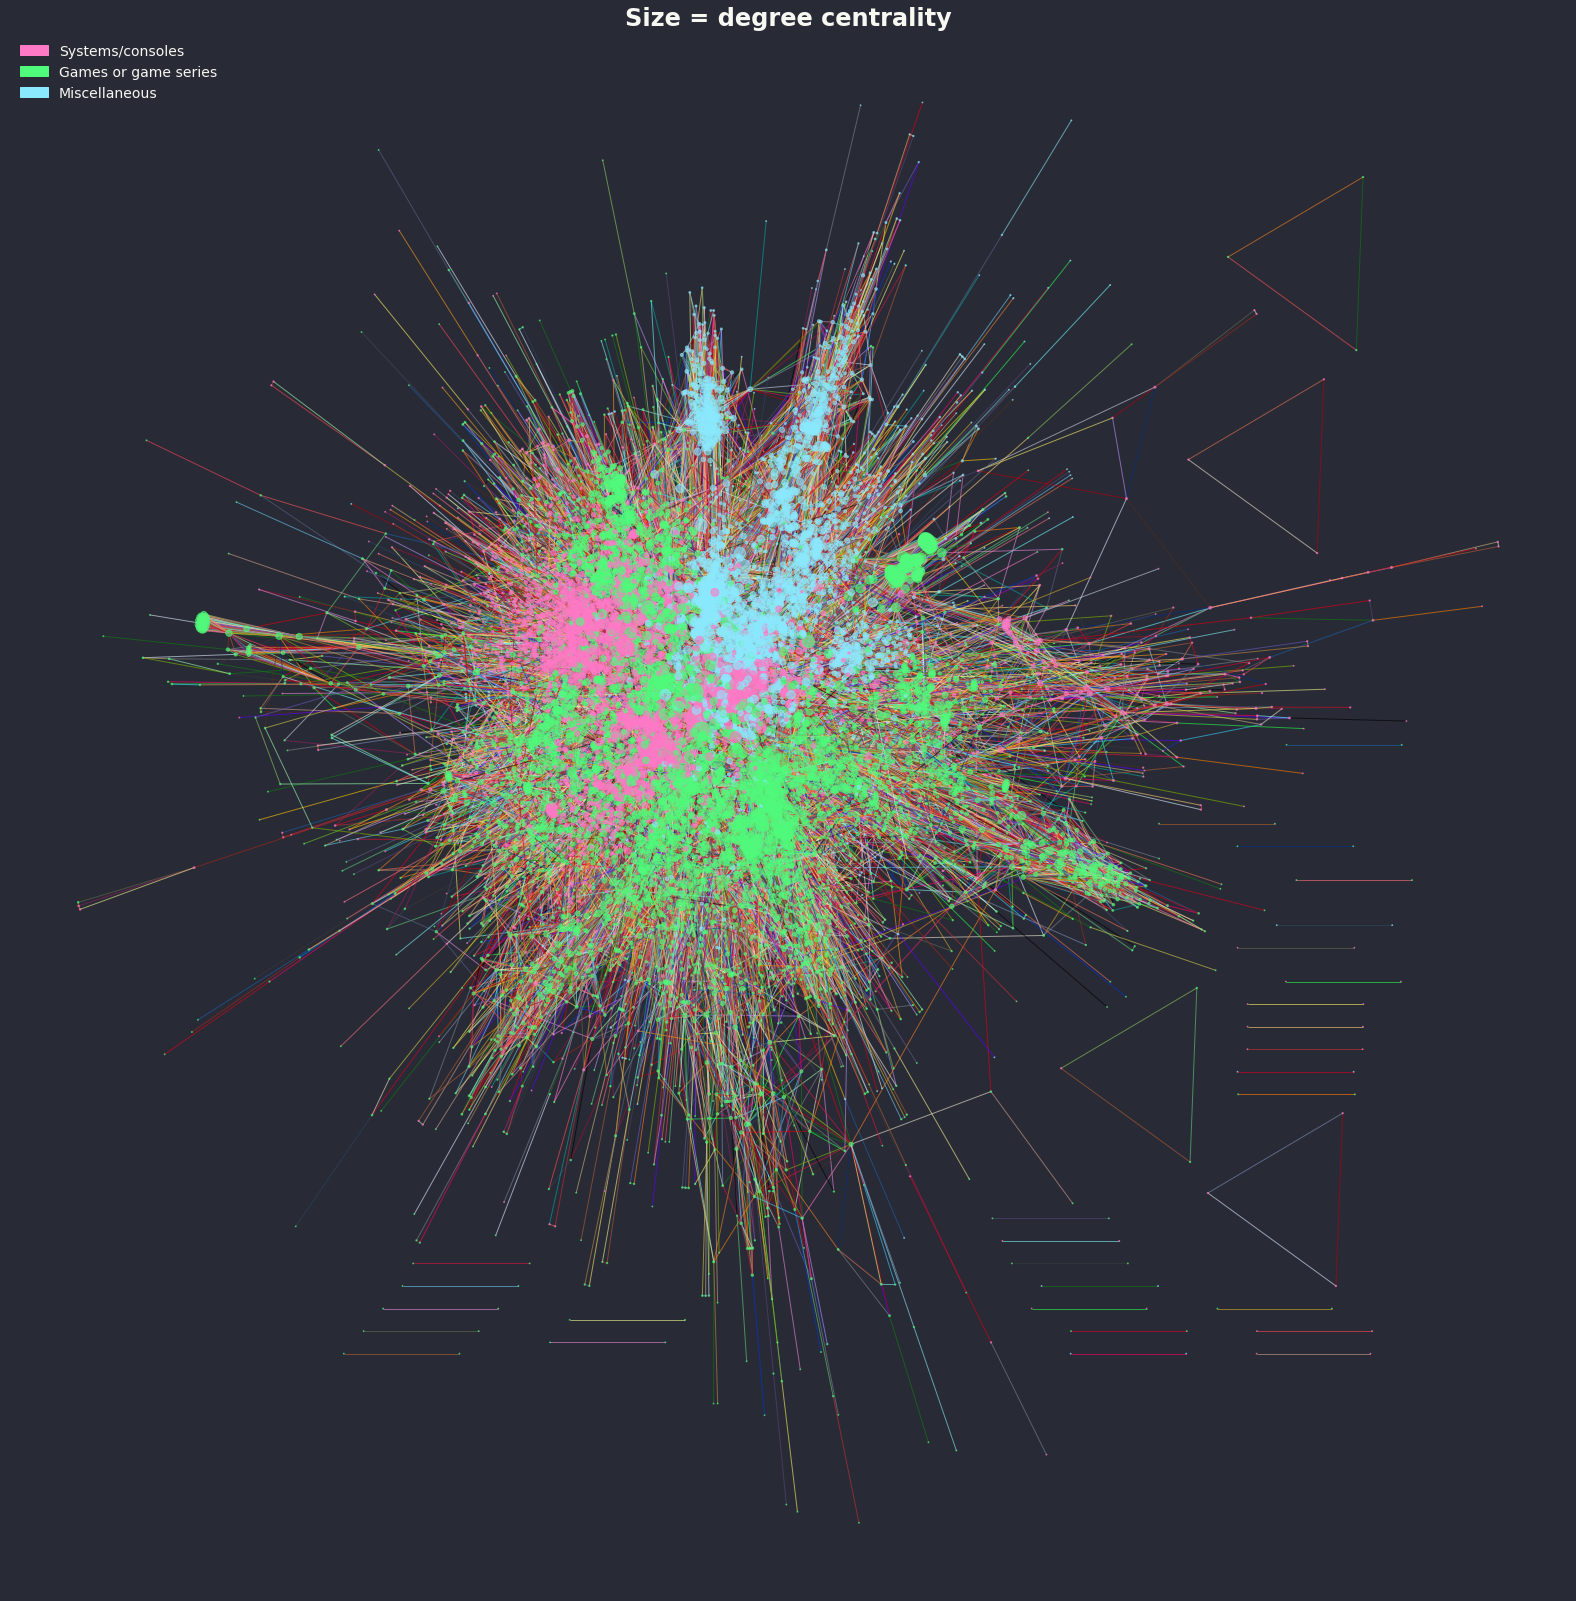
\includegraphics[width=\textwidth]{network_degcent.png}
  \caption{Full network with node sizes determined by degree centrality.}
  \label{fig:fullnet}
\end{figure}

Visualizing the full network clearly shows these disconnected nodes. The full visualization also shows the high assortativity of the SysGamGen attribute. We may observe the high connectivity as well as the diversity of edges from the plot as well. The nodes seem reasonably grouped within their assortativity class. Assortativity is 0.78 for SysGamGen and 0.75 for Systems. Both metrics are very high which \textit{may} indicate homophily in terms of sticking to the subs as they were assigned in the categories. However, as noted in limitations, the original breadth first search idea was scrapped due to computational limitations as the data grows. The high assortativity may be tautological because I lack the full picture of where those nodes posted. In other words, assortativity may be lower if data on non-gaming subs in terms of the node set were gathered. Those data would provide subs outside of the immediate gaming sphere to act as a check.

Degree assortativity is about 0.173 which is low but positive. A high correlation for degree assortativity would mean that posters tend to cluster near other Redditors with a similar degree. Thus, posters with a high degree would be expected to post in the same topics as other posters with high degrees and vice versa. The low correlation shows that degree assortativity is fairly infrequent yet not completely random. A low but nonzero correlation is sensible as some assortativity on degree is expected. For example, Redditors who post more have a greater chance of appearing in the data and likely have a higher degree which in turn means they're more likely to connect to people with other high degrees.

Density and average clustering are both low at 0.0026 and 0.033 respectively. Neither of these statistics were likely to be very high. Online social networks tend to be very dispersed rather than tightly woven. A high density would mean most Redditors responded to most posts---clearly impossible. However, low density is more conducive to information spread in terms of weak ties. Density measures connectedness which is orthogonal to information diversity. Connectivity is important (such as having an average shortest path length that isn't prohibitive to information flow), but high connectedness is not always necessary. Density is important to the extent that nodes are not isolated.

As a side note, the observed statistics were all completely outside of the boundaries of the calculated distribution of replicates. Thus, the probability of obtaining a statistic at least as extreme as what was observed is about 0 (up to 10000 replicates). P-values are not necessarily important, and low probabilities may have been a result of the algorithm used to generate the random graphs.

\begin{figure}[ht!]
  \centering
  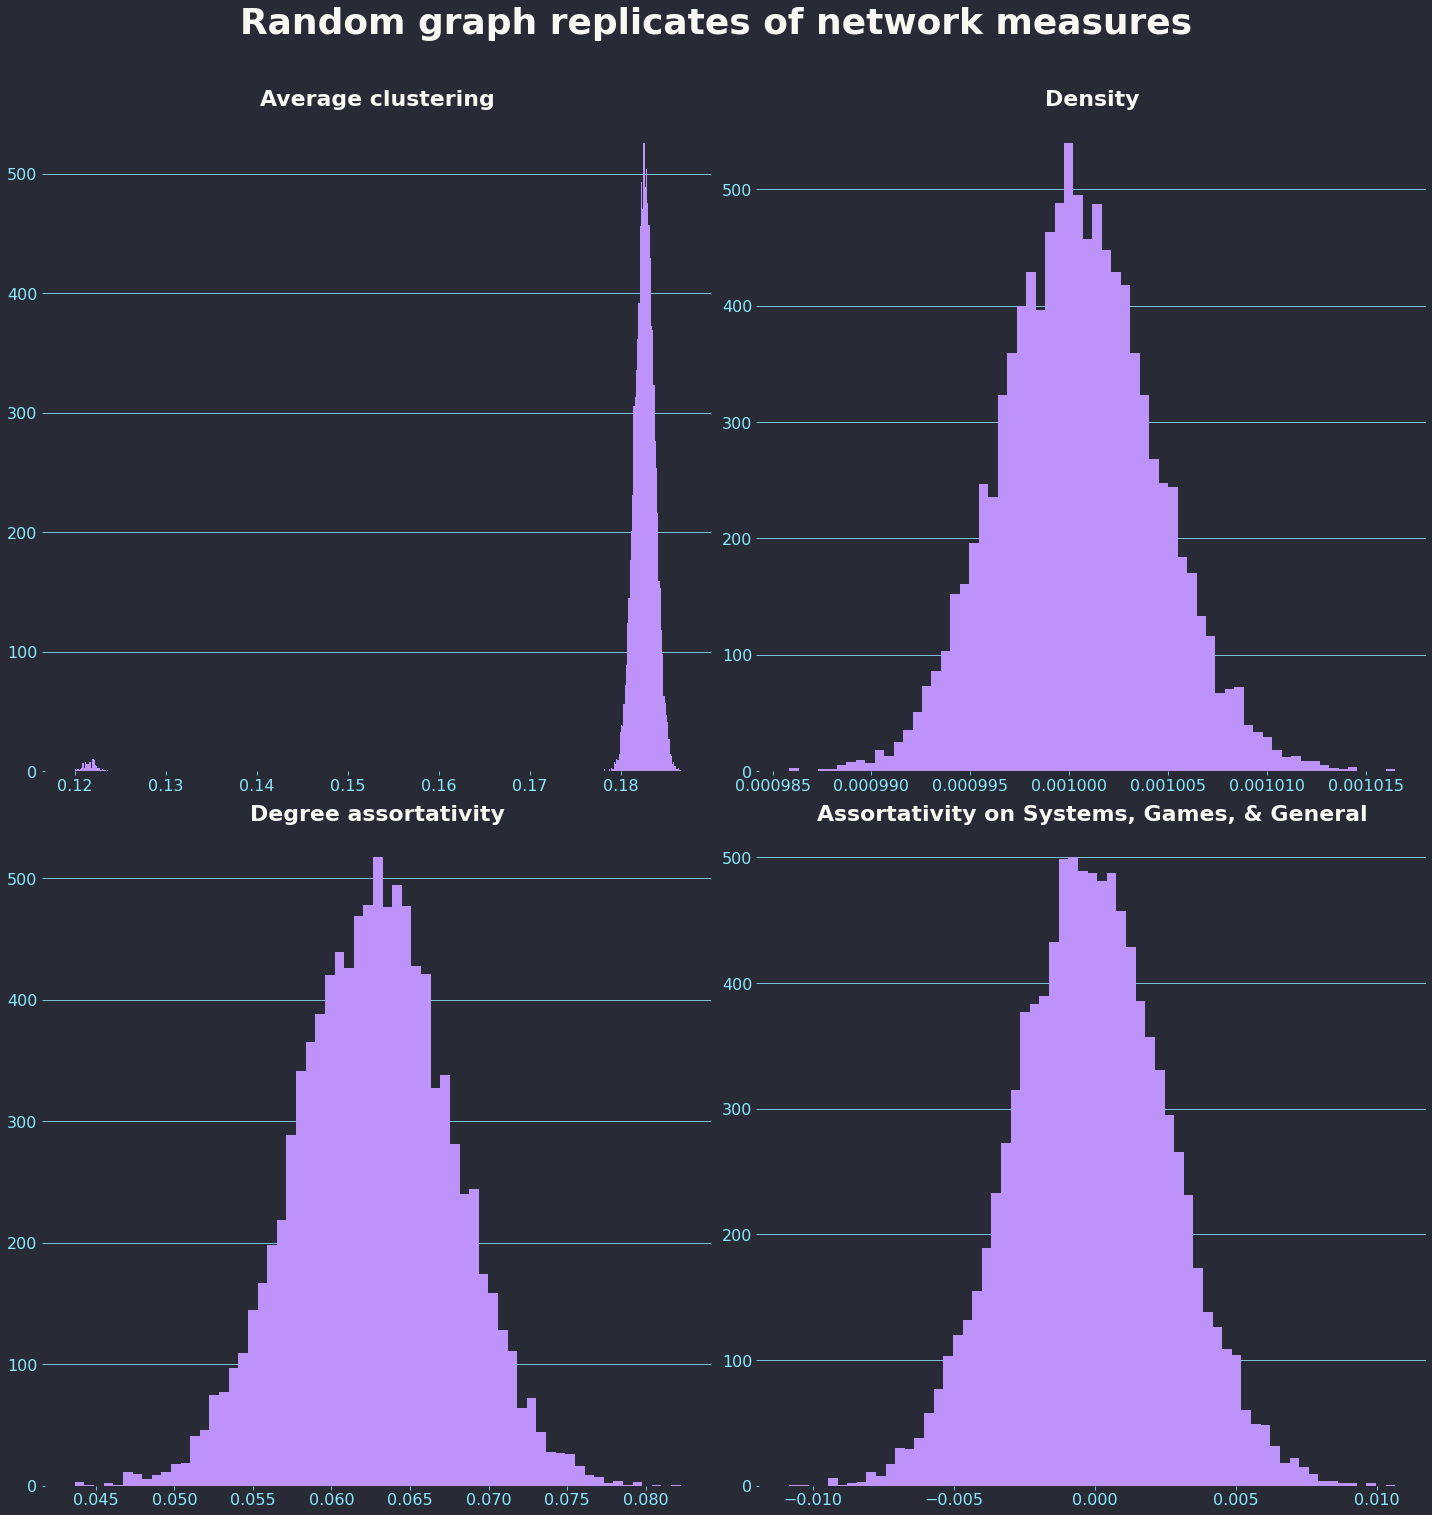
\includegraphics[width=\textwidth]{metrics_dist.png}
  \caption{Distribution of random graph replicates.}
  \label{fig:metricsdist}
\end{figure}

\begin{figure}[ht!]
  \centering
  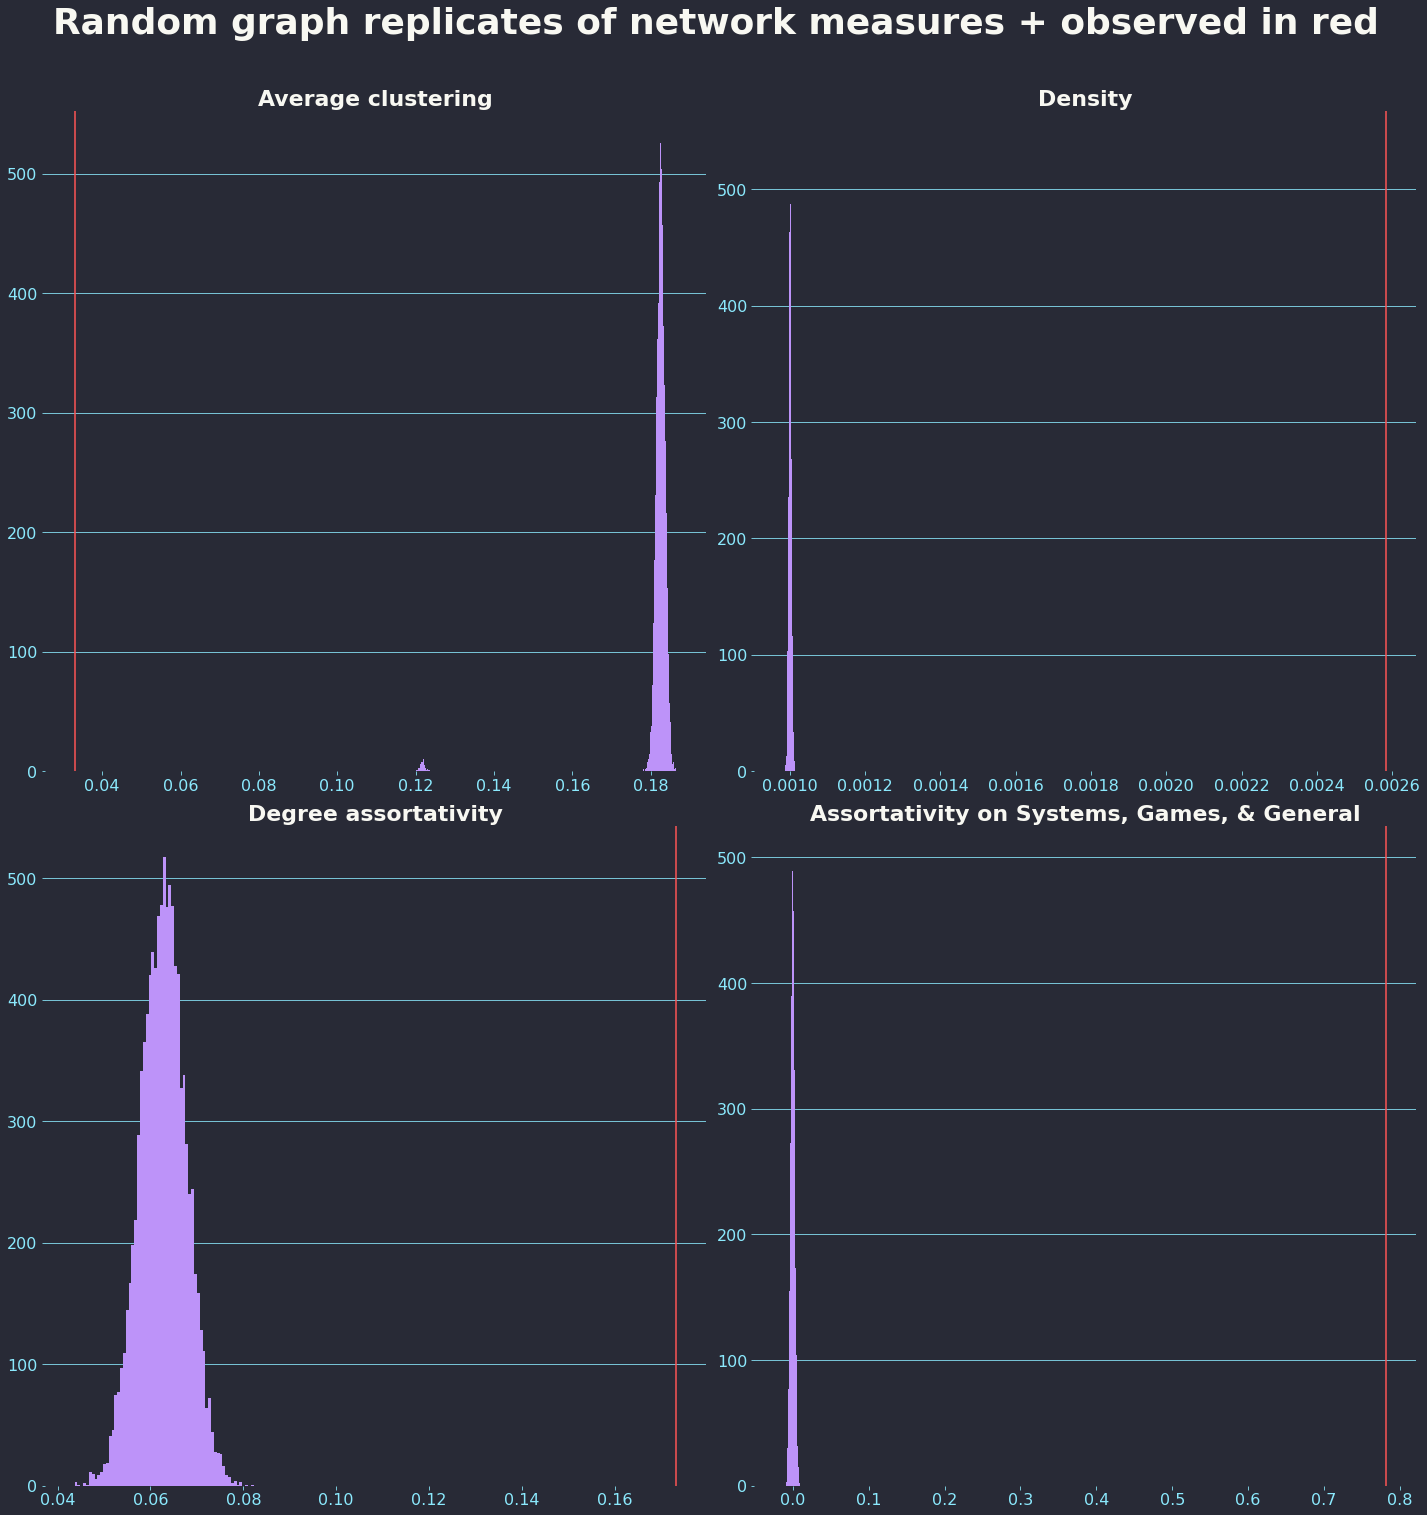
\includegraphics[width=\textwidth]{metrics_dist_w_obs.png}
  \caption{Replicates with observed statistic.}
  \label{fig:metricwobs}
\end{figure}

Both the limitations and promise of my study are demonstrated by radius and diameter. The Barycenter algorithm finds a single node in the radius while the default NetworkX center function finds 122. My data collection methodology pulled many Redditors who posted multiple times across different subs. The node with the highest unique amount of subreddits posted in at least 19 different video game related subs based on the data. NetworkX's center function detects posters who seem to be at an intersection of subreddits. One node posted in the Halo, Fall Guys, Xbox One, and Nintendo Switch subs. Fall Guys is a video game that is \textit{not} on Xbox One or the Switch. Likewise, Halo is not on the Switch. This diversity of subs likely means this node is relatively closer to other nodes (low eccentricity). Another node posted in each of the PlayStation subreddits as well as P.C. gaming's sub. Other nodes seem to have simply been lucky enough to post in pivotal topics that ensured they were closer to a variety of other nodes with connections to other subs.

\begin{figure}[ht!]
  \centering
  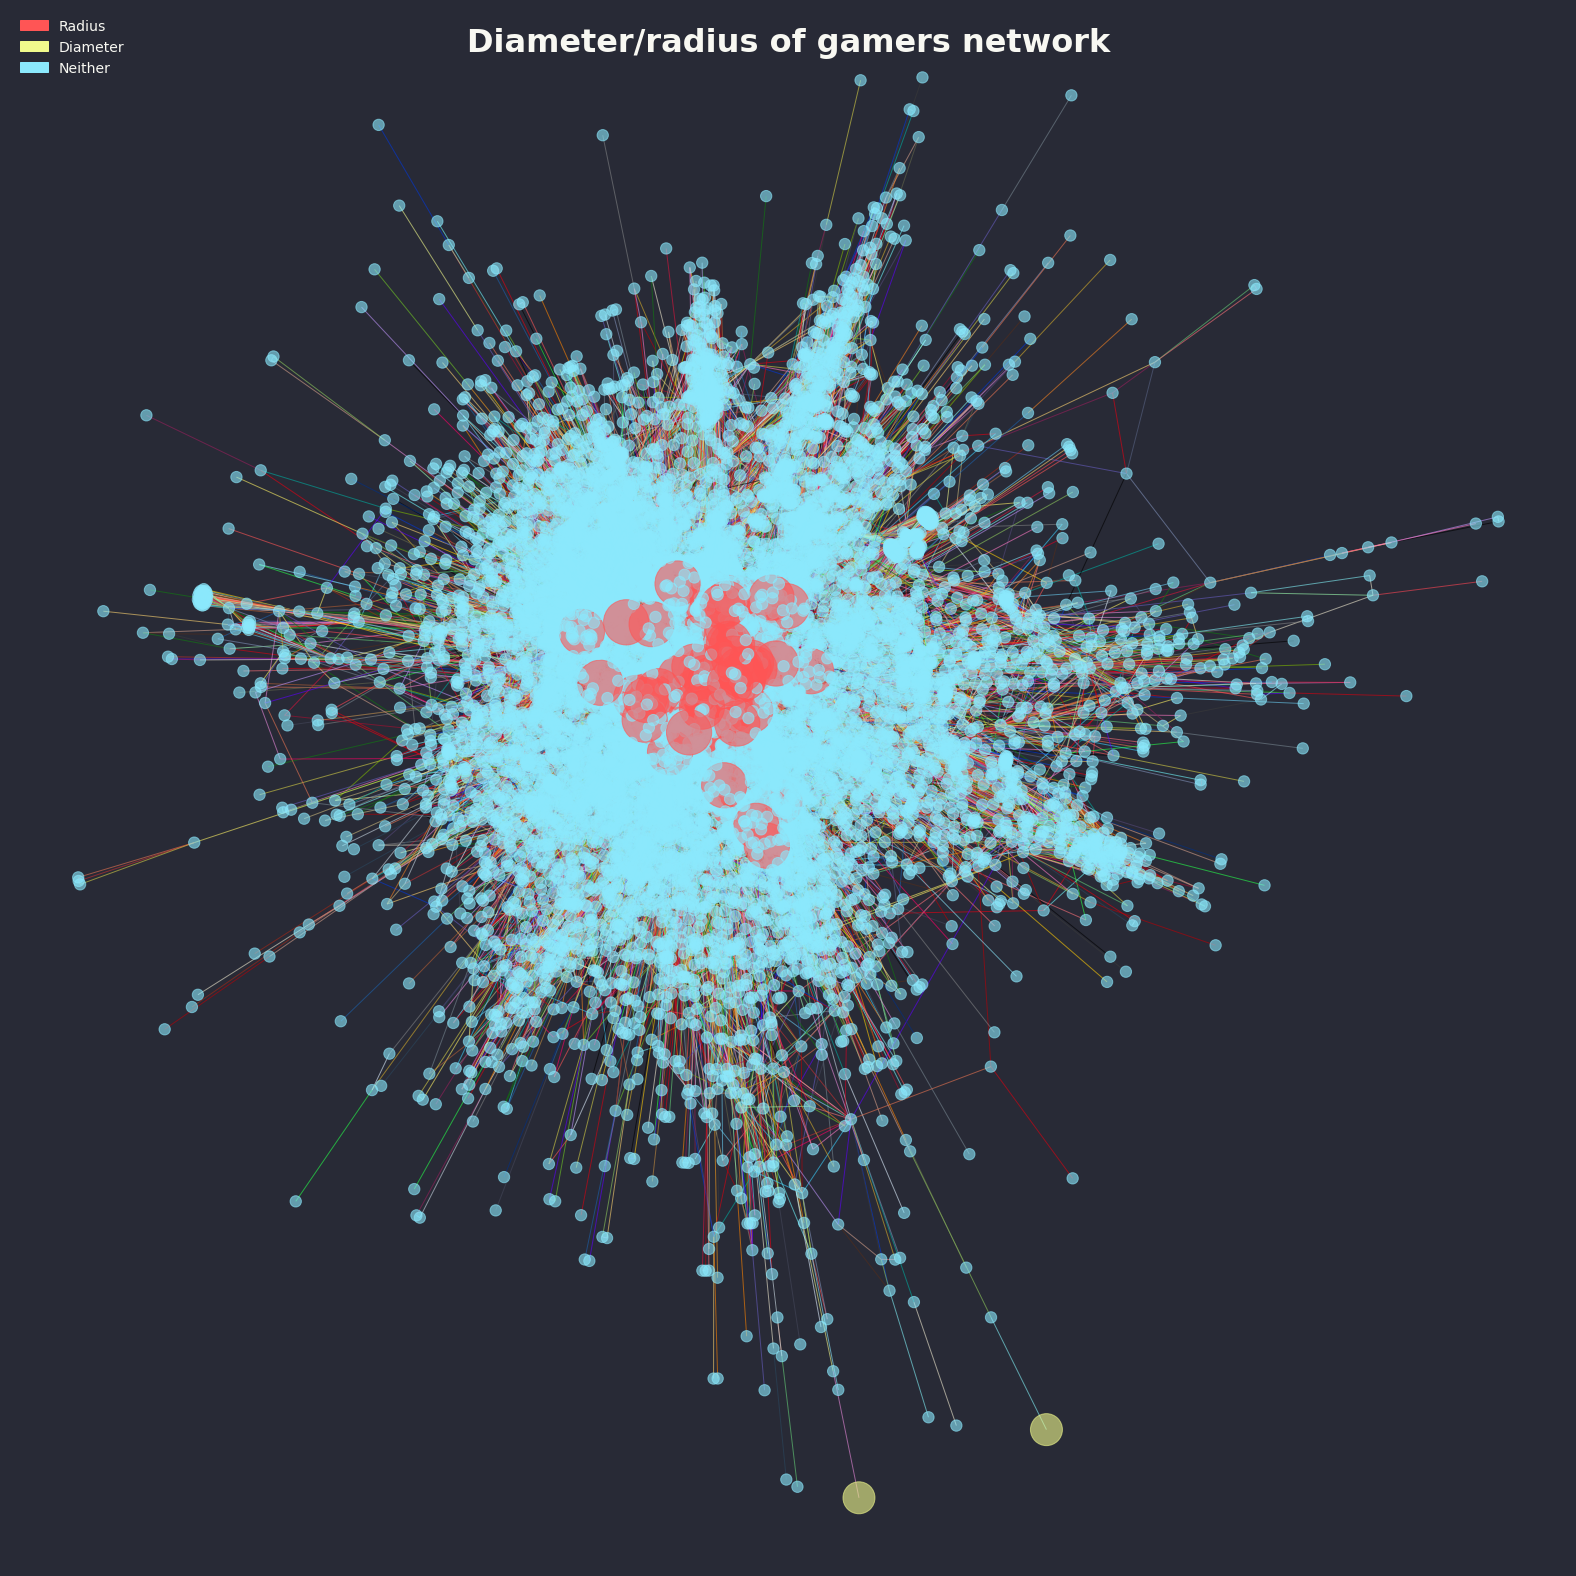
\includegraphics[width=\textwidth]{network_diarad.png}
  \caption{Diameter and radius.}
  \label{fig:diarad}
\end{figure}

The Barycenter algorithm only finds a single node in the center. Unsurprisingly, the node with the lowest eccentricity posted in 16 different video game related subreddits multiple times---and, again unsurprisingly, the subs were rather diverse. This user posted in subs associated with multiplatform gaming, P.C. gaming, games that are platform specific, as well as a couple of the humor related subs I included in my scrape. The node is not the most prevalent in my data set. In fact, many nodes occur more frequently than the node found by Barycenter. The node which appears most frequently posted 169 times. However, our most prevalent node only ever posted in the subreddit for the video game Bloodborne which is a PlayStation 4 exclusive. Bloodborne may be well received, but posting on a sub for one game that is a platform exclusive is unlikely to result in a lower eccentricity. As one would expect, the Bloodborne poster is not in the center found by the default algorithm either. While shortest path tests are too computationally expensive for my data, analyzing the center shows some evidence for information being reachable rather than more rigidly segmented.

The periphery or diameter consists of two nodes that posted a handful of times in only one subreddit. One node only posted in the Rocket League subreddit while another node only posted in the PlayStation 4 subreddit. Rocket League is a very popular competitive game which is essentially soccer with cars. The topics these two Redditors posted on have a few comments; I'll refer to these as "diameter's topics" for the rest of this paragraph. The maximum eccentricity of the graph is 11. The Redditors who posted on the diameter's topics all have eccentricities of ten. The posters on the diameter's topics, possibly due to the data's limitations, are all relatively far from the other nodes.

\begin{figure}[ht!]
  \centering
  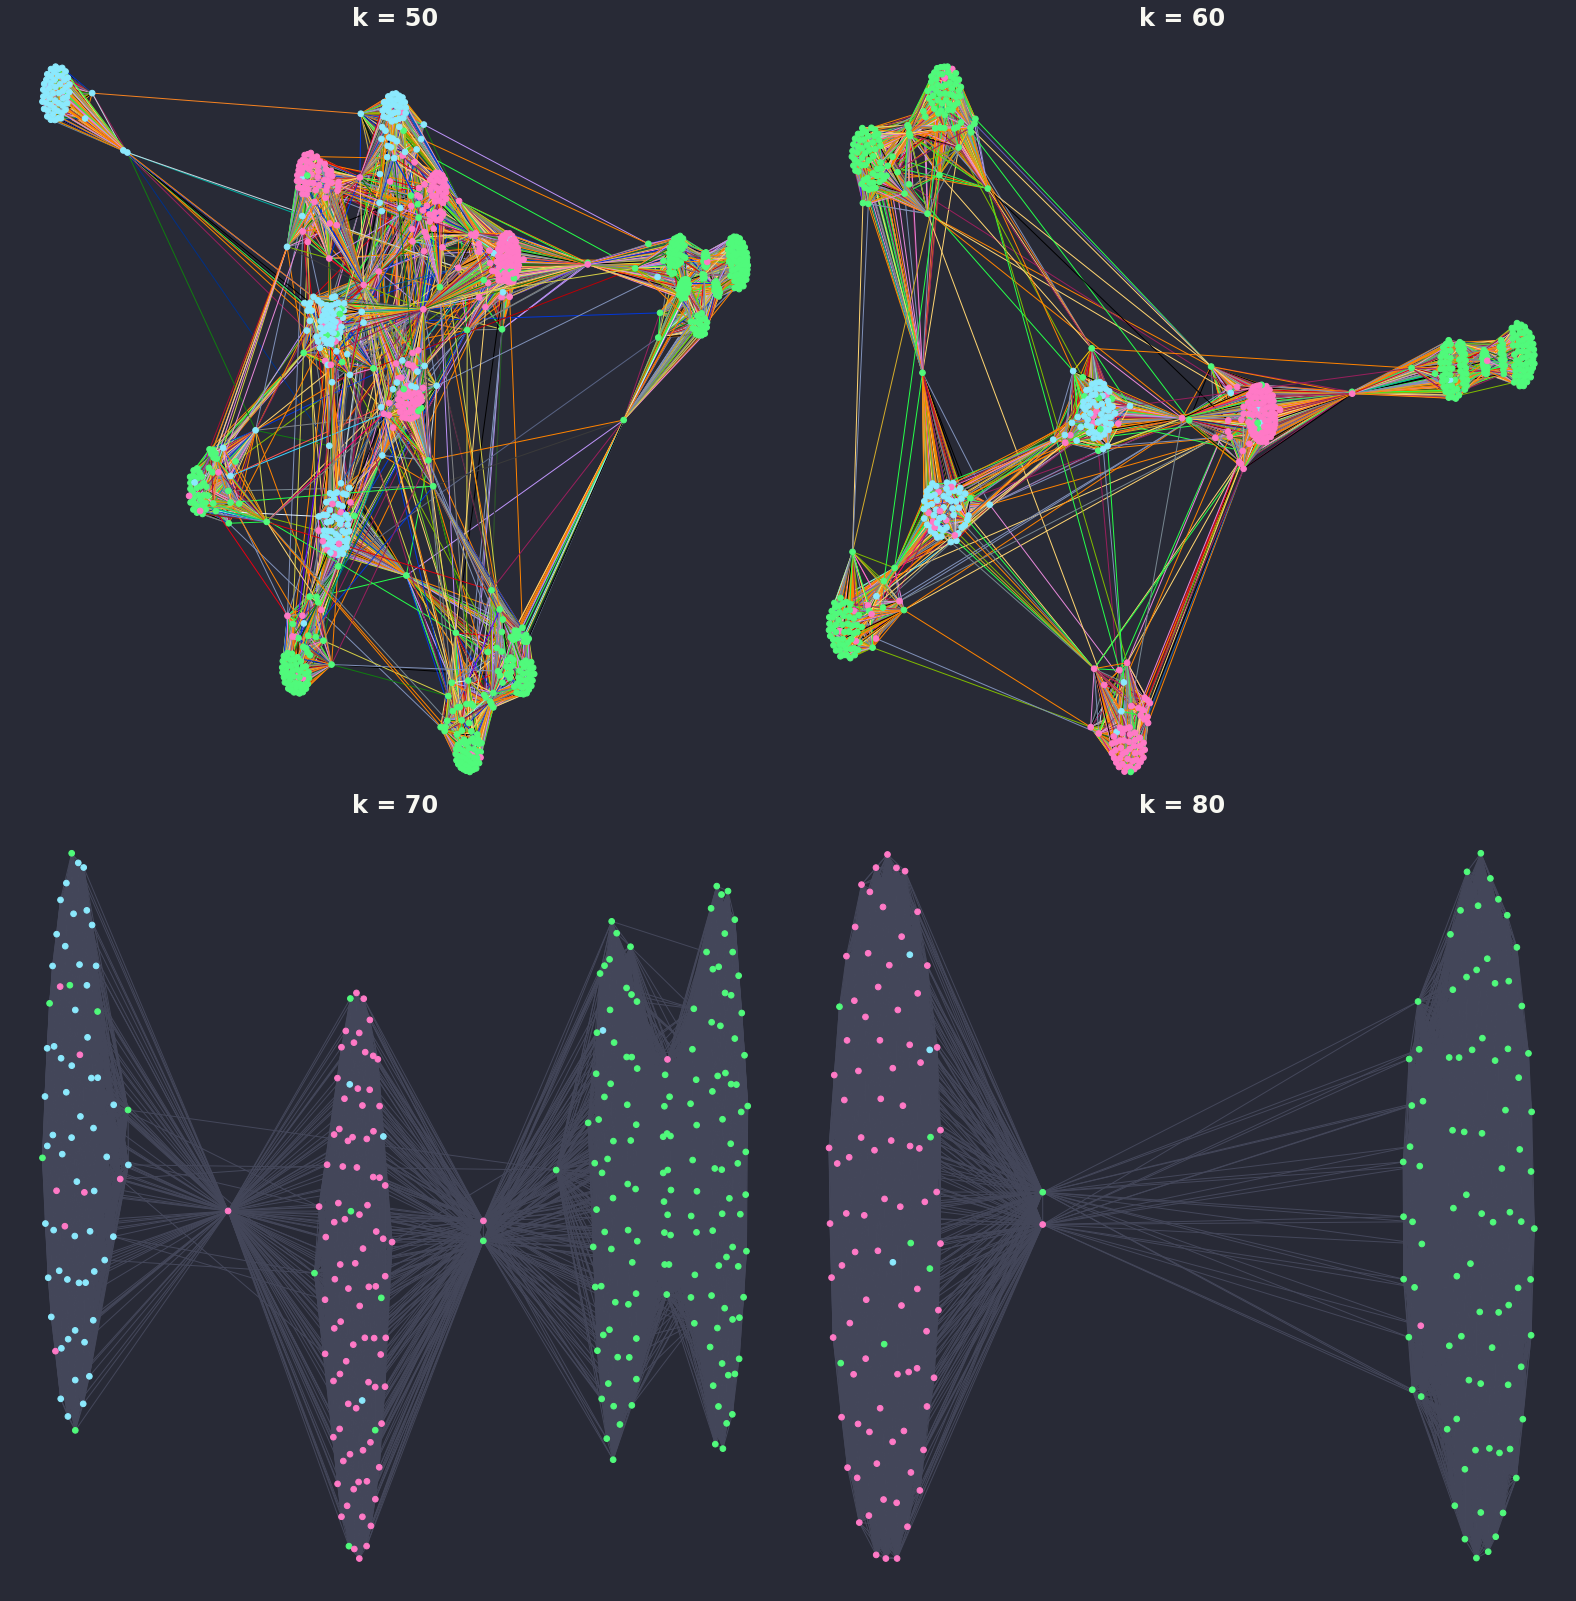
\includegraphics[width=\textwidth]{network_k_core_50_80.png}
  \caption{K-core decomposition for k 50 to 80.}
  \label{fig:kcore50_80}
\end{figure}

The k-core of a graph is a decomposition where nodes who don't meet a threshold for degree (k) are iteratively removed. The visualization above shows the k-core decomposition of the graph for k = $\{50, 60, 70, 80\}$. The graph is strongly and diversely connected despite the low density discussed earlier. A graph consisting of more data is likely to exhibit an even stronger k-core due to having more connections of course. At k = 70 and k = 80 we may notice that we have a handful of nodes that connect major sections of the decomposed graph. In both the decomposition as well as the full graph those nodes are likely to have a high betweenness centrality.

\section{Discussion}
The metrics calculated above provide evidence for the high reachability of information in the gamer's network. One way to consider this concept would be the idea of a "small world" or low hops to reach information. The small world characteristic engenders statements such as "I am six steps or less away from Obama." However, considering hops does not account for reachability. Perhaps hops two and three are far more difficult to reach than hop one on a person's quest to Obama. Network hops are likely more deterministic. For example, internet hops through routes to a web server are far different than human hops like in the Obama case. Online social networks such as Reddit are likely somewhere in between. Let's consider the node that posted in the Halo, Fall Guys, Xbox One, and Switch subs. Another Redditor, \textit{A}, who requests information that is very specific to that person's (\textit{B}) information set is more likely to receive it from \textit{B} than someone is to being connected to a stranger via the degrees of separation. The reason is that the barrier to receiving than information is far lower than the barrier to hopping human nodes through "real" connections. A person simply must ask the question in a place where a node with the requisite information set may see it. While this seems difficult when phrased that way, that just means that a node has to ask, say, some question related to Fall Guys and Xbox\footnote{Which to reiterate I realize is not on Xbox yet.} in either subreddit for example.

The limitations encountered engenders a cautious discussion. Assortativity likely requires more data so that more attributes may be designed and tested. The two attributes tested show high assortativity but a comparative approach would be superior for my research question.

\subsection{Future research}
Future research would ideally analyze much more data. My data gathering process precluded the text of the posts and topic names were encoded for privacy. However, text data, including posts and topic names, could be used for topic analysis whereby the "subjects" of each post or topic could be pulled out to use in assortativity. As mentioned earlier, more data would also mean a fuller network where more gamers can be compared across more subreddits. About a quarter of my small sample posted on at least two different subreddits, so gathering more data would likely magnify this trend. A breadth first search would result in a graph of gamers plus their posts in subreddits outside of video games. Essentially the data would consist of two separate graphs which would allow comparing the connections between gamers within gaming subreddits as well as possible connections outside of gaming subs. Finally, future research could also compare the gamer graph to graphs of music fans, sports wonks, film buffs, et cetera. Perhaps gamers are more connected across subs than Redditors interested in other topics.

Subreddits for film series as well as individual bands, musicians, and genres exist. However, none of the subreddits for these topics beyond the major subs seem to come close to gaming's efficacy. Regardless, studying a large graph of music subs comparatively with a large graph of gaming subs seems like the best step toward improving my research. The alternative graphs may function as a stronger null model in addition to the weaker p-values. A quick check shows that the subreddits for indie bands link to other indie bands as well as more encompassing subs. The subreddit for the band King Crimson links to several well known prog rock and metal subreddits as well as subs for related genres such as post-rock. However, none of these subreddits have many subscribers especially when compared to even the smaller subs gathered for this thesis.

\printbibliography

\end{document}
